

\begin{figure}
	\centering
	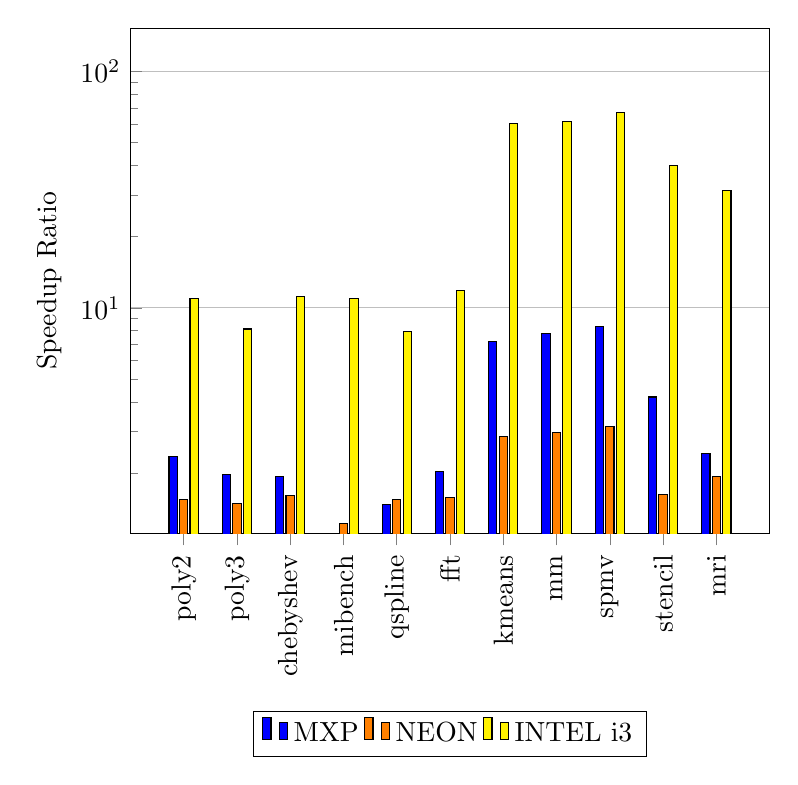
\begin{tikzpicture}
	\begin{semilogyaxis}[
	width  = 0.8*\textwidth,
	height = 8cm,
	xtick pos=left,
	ytick pos=left,
	%	major x tick style = transparent,
	x tick label style={rotate=90, anchor=east, align=right,text width=2cm},
	bar width=3pt,
	ymajorgrids = true,
	ylabel = {Speedup Ratio},
	symbolic x coords={poly2,poly3,chebyshev,mibench,qspline,fft,kmeans,mm,spmv,stencil,mri},
	xtick = data,
%	nodes near coords,
%	ybar,
%	every node near coord/.append style={rotate=90, anchor=west,font=\tiny},
	scaled y ticks = false,
	enlarge y limits={upper,value=0.2},
	%test
	%	enlarge x limits=0.25,
	ybar=2*\pgflinewidth,
	legend cell align=left,
	legend style={
		at={(.5,-0.35)},
		anchor=north,
		legend columns=-1
		column sep=0.5ex
	}
	]
	\addplot[draw=black,fill=blue]
	coordinates {(poly2,2.35) (poly3,1.98) (chebyshev,1.933) (mibench,1.11) (qspline,1.47) (fft,2.033) (kmeans,7.20) (mm,7.779) (spmv,8.32) (stencil,4.20) (mri,2.42) };
	
	\addplot[draw=black,fill=orange]
	coordinates	{(poly2,1.55 ) (poly3,1.49) (chebyshev,1.61) (mibench,1.22) (qspline,1.55) (fft,1.58) (kmeans,2.86) (mm,2.98) (spmv,3.16) (stencil,1.63) (mri,1.934) };
	
	\addplot[draw=black,fill=yellow]
	coordinates	{(poly2,11 ) (poly3,8.14) (chebyshev,11.13) (mibench,10.97) (qspline,7.95) (fft,11.85) (kmeans,60.42) (mm,61.53) (spmv,67.023) (stencil,40.039) (mri,31.28) };
	
	\legend{MXP,NEON,INTEL i3}
	\end{semilogyaxis}	
	\end{tikzpicture}
	\caption{Word level Speedup Analysis w.r.t ARMv7 for  different benchmarks.}
	\label{speedup:3}
\end{figure}
